\documentclass[reprint,amsmath,amssymb,aps,]{revtex4-2}
\usepackage{graphicx}
\usepackage{dcolumn}
\usepackage{bm}
\usepackage{scrextend}
\usepackage{vmargin}
\usepackage{multirow}
\usepackage[utf8]{inputenc}
\usepackage[spanish, es-tabla]{babel}
\usepackage{enumerate}
\usepackage{float}
\usepackage{subcaption}
\usepackage{lipsum}
\usepackage{amsmath, amsthm, amssymb, amsfonts}
\usepackage[usenames]{color}
\usepackage[breaklinks=true,hidelinks]{hyperref}
\pagestyle{empty}
\spanishdecimal{.}
\begin{document}
\preprint{APS/123-QED}
\begin{abstract}
La estrucuta periódica de un sólido cristalino actúa como una red de difracción, dispersando los electrones de una manera predecible. Trabajando a partir del patrón de
difracción observado, puede ser posible deducir la estructura cristalina que produce el patrón de difracción. En este reporte se obtuvo las posiciones de varios átomos difractados
a partir de una simulación, se creo un algoritmo en python, el cual, a partir de las posiciones de los átomos se reconoce que distancias interatomicas guardar y
asociarlas a una familia de indices de Miller dada.
\end{abstract}
\begin{titlepage}
\begin{center}

\includegraphics[scale=0.40]{../../../Logos/uanl.png} 
\hspace{2.5cm}

\includegraphics[scale=0.40]{../../../Logos/fcfm.png}
\end{center}
\vspace{2cm}
\begin{center}
\textbf{
UNIVERSIDAD AUTÓNOMA DE NUEVO LEÓN\\
FACULTAD DE CIENCIAS
FÍSICO MATEMÁTICAS}\\
\vspace*{2cm}
\begin{large}
\vspace{1cm}
\large{\textbf{Aplicaciones de la Mecánica Cuántica}}\vspace{1.5cm}\\
\textbf{Reto 2}\\
Carlos Luna\\
\end{large}
\vspace{3.5cm}
\begin{minipage}{0.6\linewidth}
\vspace{0.5cm}
\changefontsizes{14pt}
Nombre:\\
Giovanni Gamaliel López Padilla\\
\end{minipage}
\begin{minipage}{0.2\linewidth}
\changefontsizes{14pt}
Matricula:\\
1837522\\
\end{minipage}
\end{center}
\vspace{4cm}
\begin{flushright}
\today
\end{flushright}
\pagebreak
\end{titlepage}
\maketitle
\section{Introducción}
La difracción de electrones es una t\'ecinca usada para estudiar la 
materia a partir del patr\'on  de interferencia, esto con la finalidad de 
analizar la estructura cristalina de los s\'olidos, los principios físicos en los cuales se basa es la 
dispersión o difracción de Bragg. En 1912, W. Friedrich y P. Knipping realizaron un experimento el cual consistia en
hacer pasar un haz colimado de rayos X a través de un cristal detrás del cual había colocadouna fotografía, además de esta Configuración
se colocó un haz central que corresponde a la dirección incidente observando una distribución regular de puntos. Este patrón fue explicado por los mismos autores
del experimento, a dicho fenomeno se le denomino dispersión de Bragg. Los experimentos se realizan comunmente en los microscopios electrónico de transmisión (TEM)
,o un microscopio electrónico de barrido (SEM). En estos instrumentos, los electrones son acelerados por un potencial electrostático para obtener la energía deseada
y determinar su longitud de onda antes de que interactúen con sla muestra a estudiar. 
\section{Objetivo}
\begin{itemize}
    \item Realizar una transformada de Fourier (FFT) de la nanopartícula capturada.
    \item Indexar la imagen FFT e identificar las caras cristalinas expuestas de la nanopartícula.
    \item Determinar la dirección cristalográfica en la que se esta estudiando la nanopartícula.
\end{itemize}
\section{Marco teórico}
La difracción de electrones se basa en la teoría cuantica de la dualidad onda-partícula. El haz de electrones se comporta como un conjunto
de ondas que inciden sobre el material cristalino y se difractam en los centros de dispersión, lugares donde la densidad electrónica es más alta
esto quiere decir que en esa posición es más probable de encontrar a los átomos que conforman el material.\\ 
La difracción de electrones es una técnica muy utilizada en Física de Materiales. La estructura periódica
de un sólido cristalino actúa como una red de difracción para los electrones, pues la longitud de onda de
los electrones tiene un tamaño parecido al espaciado interatómico. Esto lo convierte en una buena
alternativa a la difracción de rayos X para
estudiar la estructura cristalina de los
materiales. En cada caso, los electrones cumplen una relación de interferencia constructiva distinta, aunque todos
ellos son muy similares a la relación del ejercicio (donde, por simplicidad, en lugar de un material, se
trata una cadena monoatómica con distancia interatómica similar al parámetro de red del Si) y se
obtienen de la misma forma: a partir de imponer que la diferencia de caminos entre los haces
difractados sea igual a un número entero de longitudes de onda. Se pueden sacar conclusiones del
ejercicio válidas para todos los casos: los patrones son simétricos en torno a $\theta$=0 y $sin(\theta)$ es
inversamente proporcional al parámetro de red a y proporcional a la raíz cuadrada de la energía de los
electrones incidentes.\\
Para este caso tenemos un material de oro, este material cristalino cumple con los parámetros 
mostrados en la tabla \ref{tabla:parametros}.
\begin{table}[H]
    \centering
    \begin{tabular}{ccccc}\hline
        2$\theta$ & Intensity & D-Spacing (\r{A}) & HKL & Multiplicity\\ \hline
        38.15 & 100 & 2.3592 & 111 & 8 \\
        44.34 & 46.77 & 2.0431 & 200 & 6 \\
        66.50 & 25.61 & 1.447 & 220 & 12 \\
        77.47 & 27.18 & 1.2320 & 311 & 24 \\
        81.62 & 7.69 & 1.1796 & 222 & 8 \\ \hline
    \end{tabular}
    \caption{Parámetros para las difracciones de una nanopartícula de oro.}
    \label{tabla:parametros}
\end{table}
Al realizar la difracción de electrones obtenemos una imagen de la partícula la cual nos da información acerca de la forma que puede tener. \\
Al aplicar una transformada de Fourier a esta imagen, no arrojada las posiciones en donde existe una mayor densidad de difracción de electrones, los cuales podemos interpretar como las posiciones de los átomos
de la estructura cristalina.
\section{Resultados}
La nanopartícula de oro estudiada es la que se muestra en la figura \ref{fig:nanoparticula}. Esta se encuentra a una resolución de 10 nm,
la primera impresión que da la imagen es que se trata de una nanopartícula esferica, ya que, las sombras que capto el microscopio electrónico
lo muestran.
\begin{figure}[H]
    \centering
    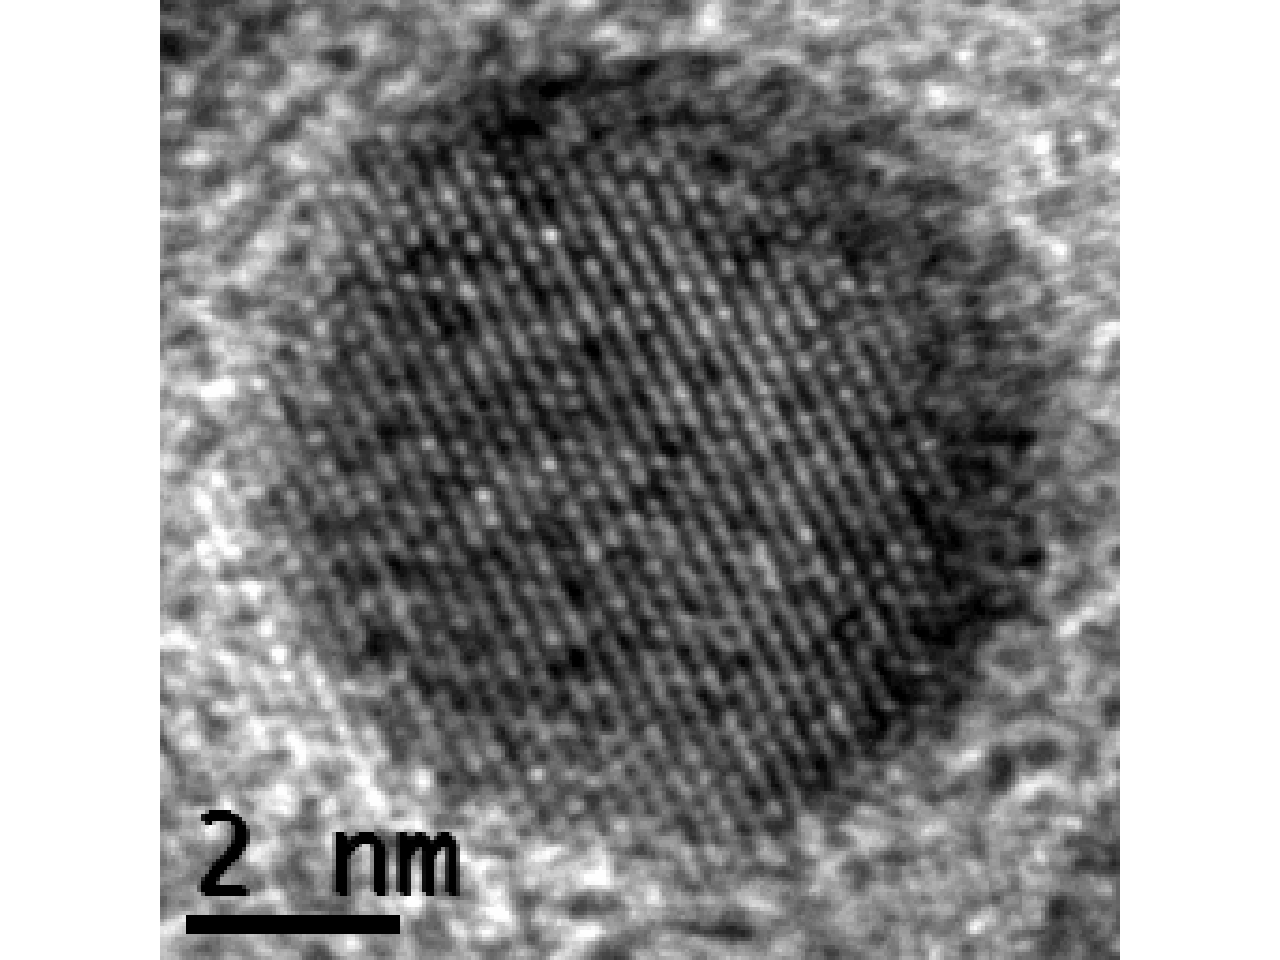
\includegraphics[scale=0.45]{../Graphics/Original.png}
    \caption{Nanopartícula de oro a una resolución de 10 nm.}
    \label{fig:nanoparticula}
\end{figure}
Para realizar un análisis a profundidad de la nanopartícula se procedio a aplicarle una Transformación de Fourier a la imagen, esto es para obtener 
las posiciones donde hubo una mayor difracción de electrones. Este procedimiento se realizó por medio de un código propietario escrito en el lenguaje python.
Este programa lee la figura \ref{fig:nanoparticula} y realiza la siguiente operación:
\begin{equation}
    \changefontsizes{9pt}
    X_k = \sum_{n=0}^{N-1} x_n e^{-j2\pi kn/N} , k=0,1,\cdots > N-1
    \label{eq:dft}
\end{equation}
Al resultado de la transformada se le realizo un filtrado de los coeficientes espectrales iguales a cero para que estos valores tuvieran su posición en el centro de la imagen.
Ya con este proceso se calculo la norma de cada vector, ya que la transformada de Fourier nos puede arrojar valores complejos, y para obtener la magnitud de las frecuencias se le aplico
una función logaritmo. Con este proceso realizado obtenemos la figura \ref{fig:fft}.
\begin{figure}[H]
    \centering
    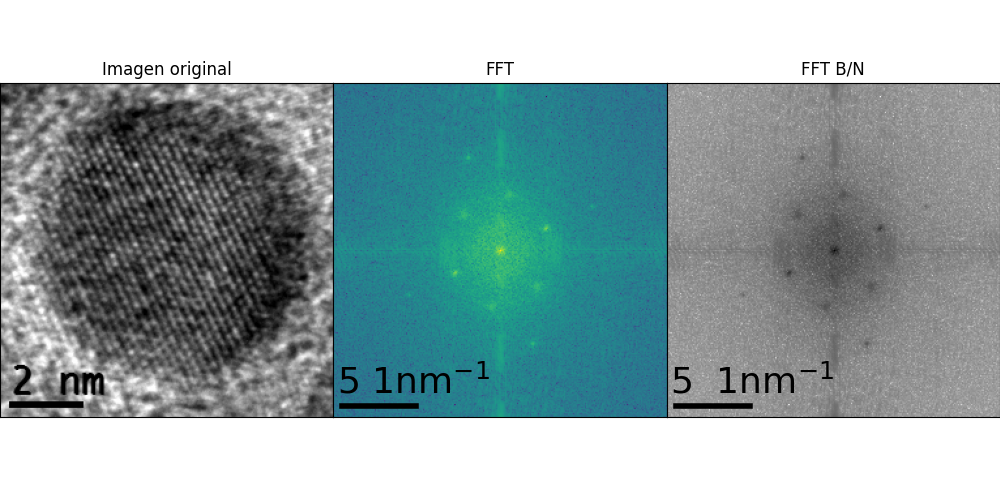
\includegraphics[scale=0.4]{../Graphics/FFT.png}
    \caption{Transformada de Fourier de la figura \ref{fig:nanoparticula}.}
    \label{fig:fft}
\end{figure}
Realizando una Transformación a la figura \ref{fig:fft} para obtenerla en la escala de grises, se obtuvó la figura \ref{fig:fftbn}.
\begin{figure}[H]
    \centering
    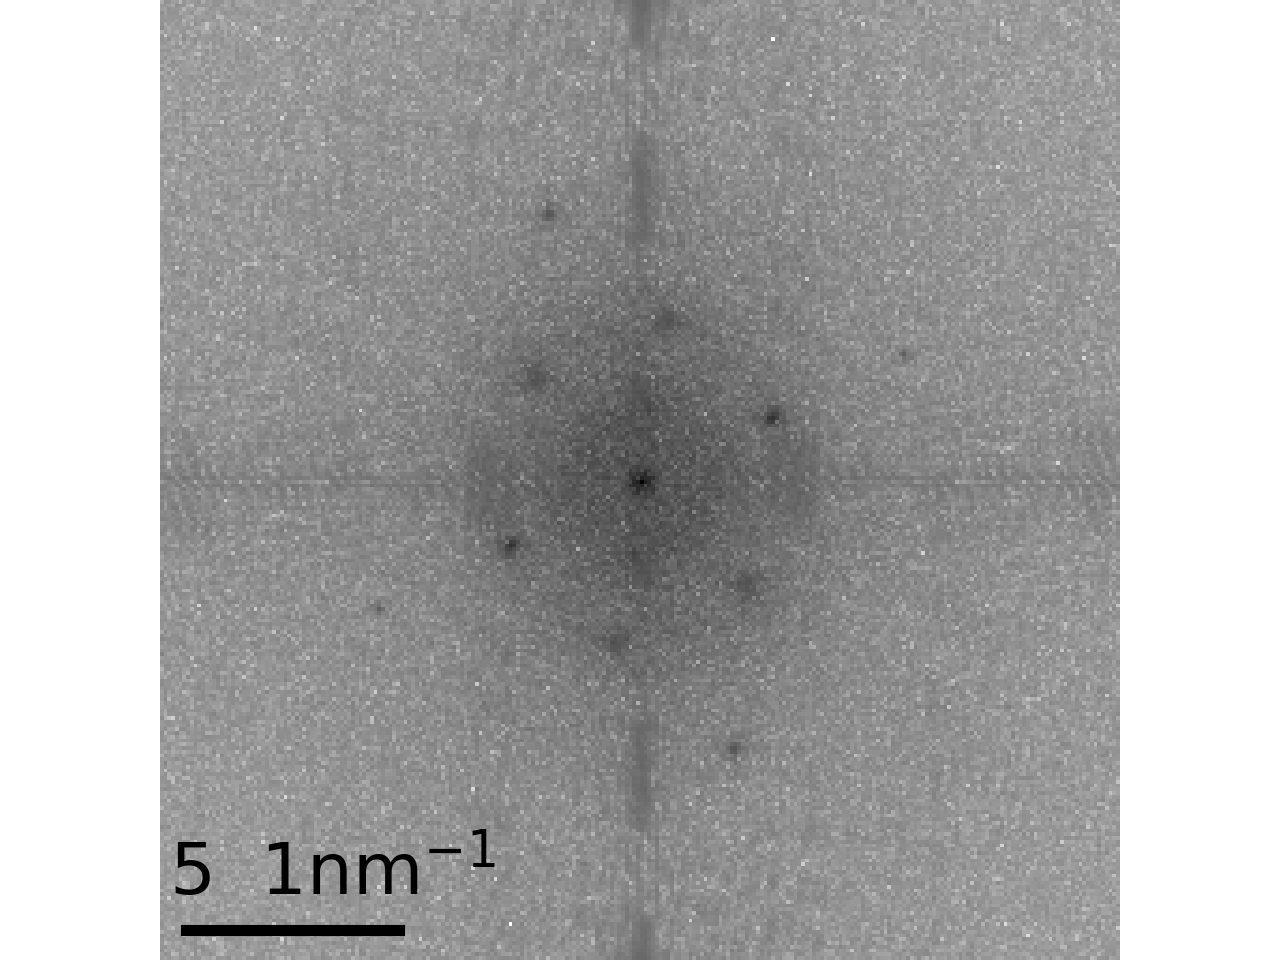
\includegraphics[scale=0.4]{../Graphics/FFTBN.png}
    \caption{Escala de grises de la figura \ref{fig:fft}}
    \label{fig:fftbn}
\end{figure}
A partir de la figura \ref{fig:fftbn}, se obtuvieron las posiciones de cada difracción en el espacio recíproco. Estas posiciones fueron guardadas en un archivo de datos para 
calcular las distancias entre puntos, las cuales serán comparadas con la tabla \ref{tabla:parametros} y así realizar la asignación de los indices de Miller correspondiente a cada punto.\\
 Los puntos recolectados son los mostrados en la figura \ref{fig:puntosiniciales}.\\
 Se definieron una serie de condiciones para que el programa decida que distanicas entre puntos tomara encuenta para la asignación de cada inidice de Miller.
 Las condiciones que se impusieron son las 
siguientes:\\
Se definio al centro de la imagen como el órigen, por lo que al tomar dos puntos A y B, sus distancias serán guardadas si y solo si:
\begin{itemize}
   \item La diferencia entre la distancias hacia el centro de cada punto es menor a 8.75 pixeles.
   \item La diferencia entre las pendientes de la recta de cada punto hacia el origen es menor a 1.7.\\
   \item Los signos de las pendientes sean los mismos. 
\end{itemize}
 \begin{figure}[H]
     \centering
     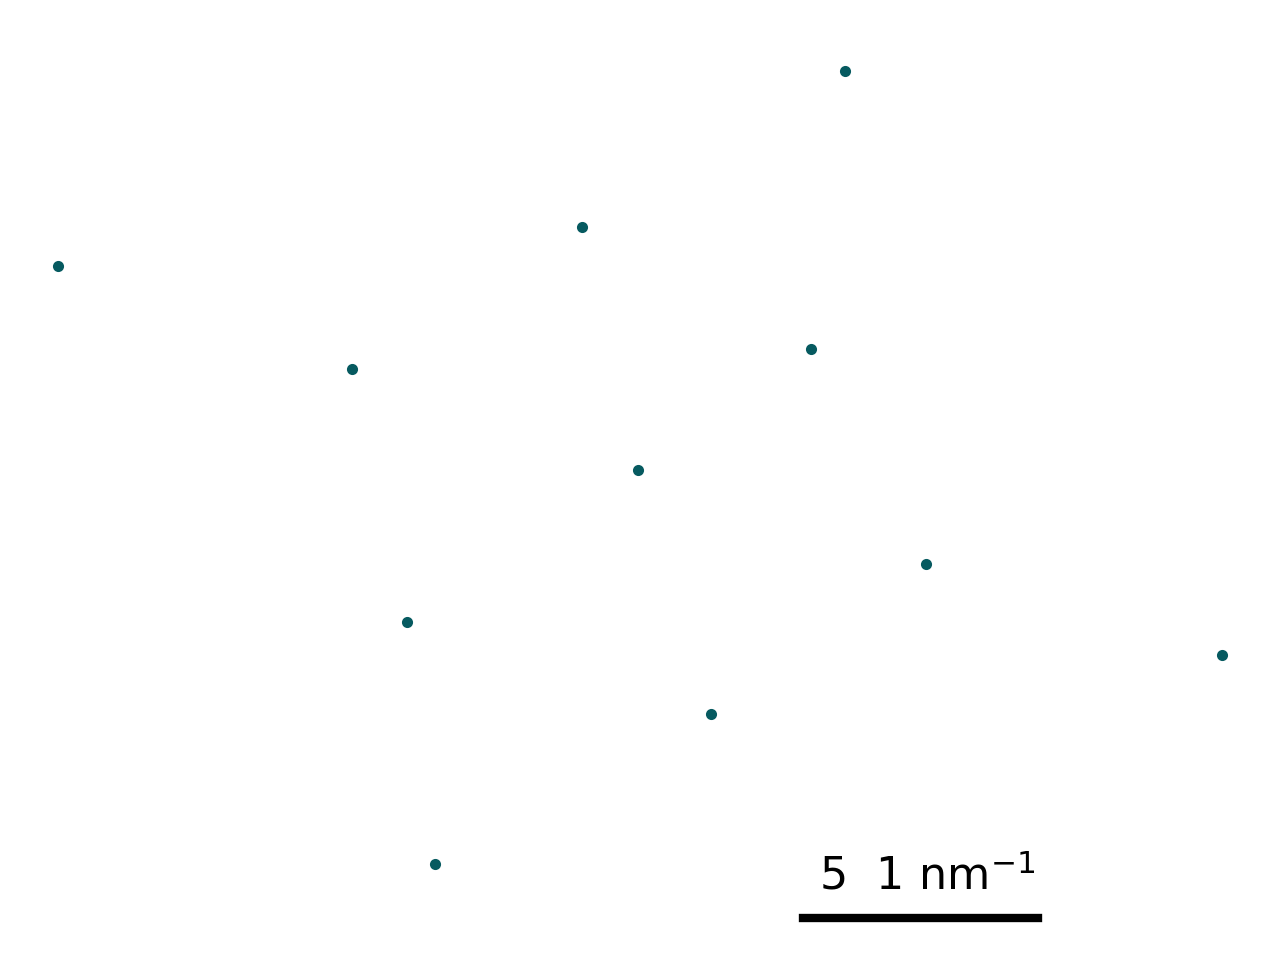
\includegraphics[scale=0.4]{../Graphics/inicial.png}
     \caption{Puntos de difracción recolectados de la figura \ref{fig:fftbn}}
     \label{fig:puntosiniciales}
 \end{figure}
Con esto definido, el algoritmo realizo la siguiente selección de distancias entre puntos de difracción:
\begin{figure}[H]
    \centering
    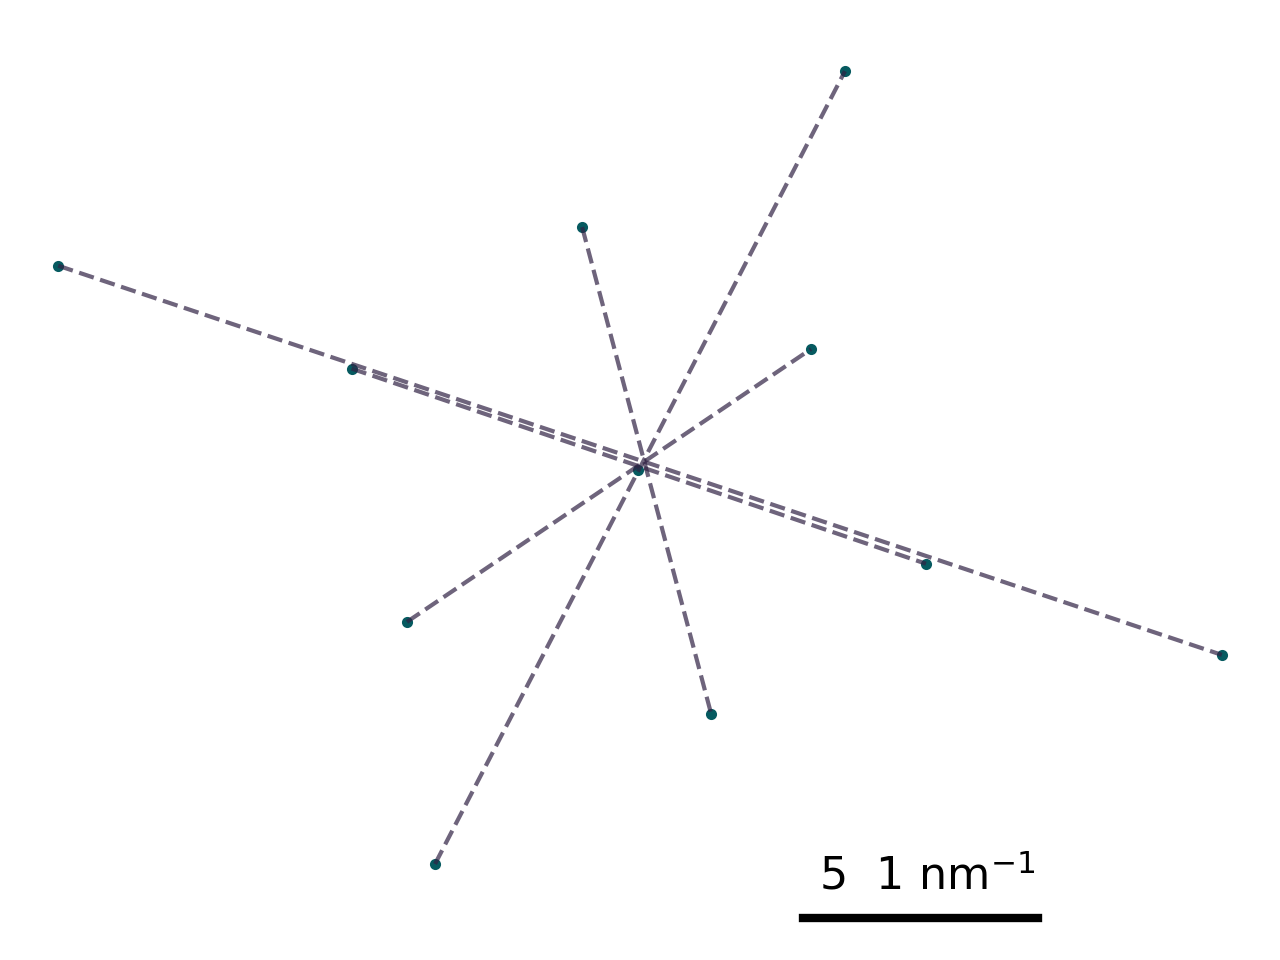
\includegraphics[scale=0.4]{../Graphics/distancia.png}
    \caption{Distancias entre puntos de dispersión de electrones obtenida a partir de las condiciones impuestas en el algoritmo y las posiciones mostradas en la figura  \ref{fig:puntosiniciales}}
    \label{fig:distancias}
\end{figure}
Con esta información se realizaró la asignación de cada familia de indices de Miller asociado a cada punto, la asignación fue realizada por otro algoritmo, el cual al calcular la diferencia entre las distacias mostradas en la tabla
\ref{tabla:parametros} este asignaba un indice de Miller correspondiente, por lo tanto, los inidices de Miller para cada punto es la siguiente:
\begin{figure}[H]
    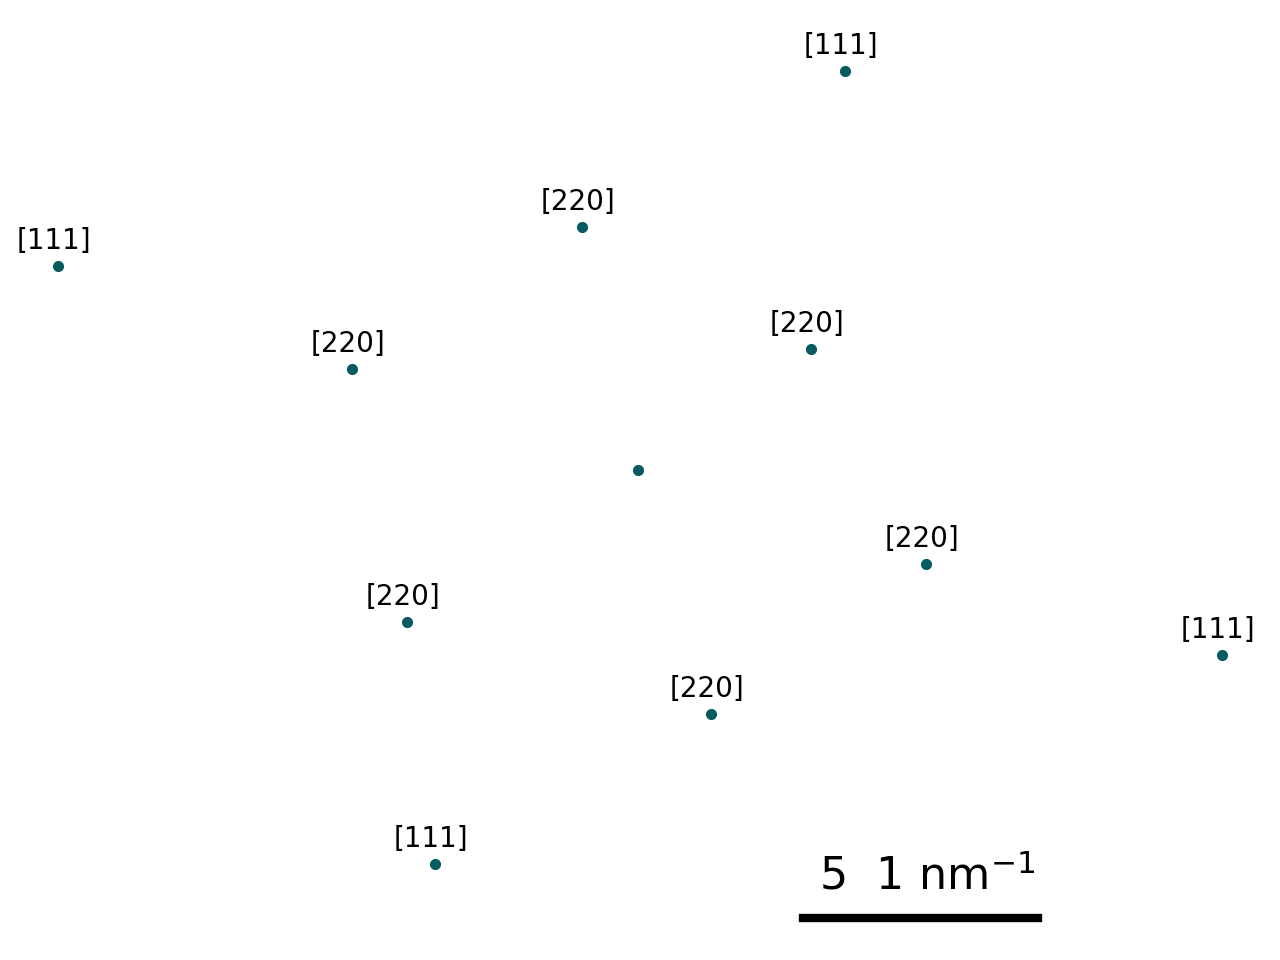
\includegraphics[scale=0.4]{../Graphics/indices.png}
    \caption{Familia de indices de Miller para cada punto a partir de las distancias mostradas en la figura \ref{fig:distancias} y los valores de la tabla \ref{tabla:parametros}.}
    \label{fig:indices}
\end{figure}
Realizando el cálculo de los indices de Miller para cada punto a partir de su familia, se encontraron los siguientes:
\begin{figure}[H]
    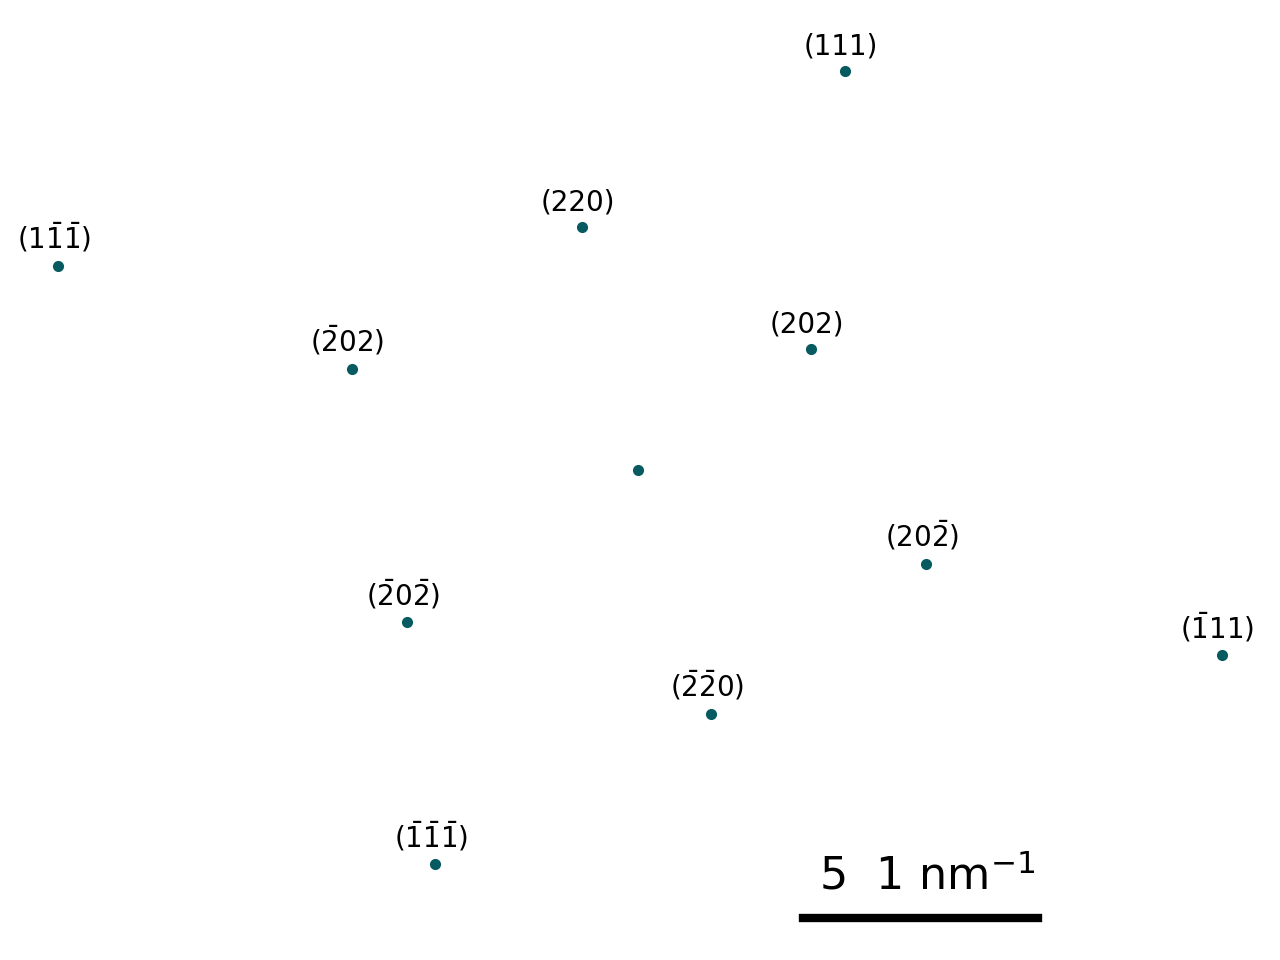
\includegraphics[scale=0.4]{../Graphics/lattice.png}
    \caption{Indices de Miller asignados a partir de la familia encontrada en la figura \ref{fig:indices}}
    \label{fig:lattice}
\end{figure}
Superponiendo los indices de Miller en cada punto con la transformada de Fourier de la figura \ref{fig:fft}, se obtuvo lo siguiente:
\begin{figure}[H]
    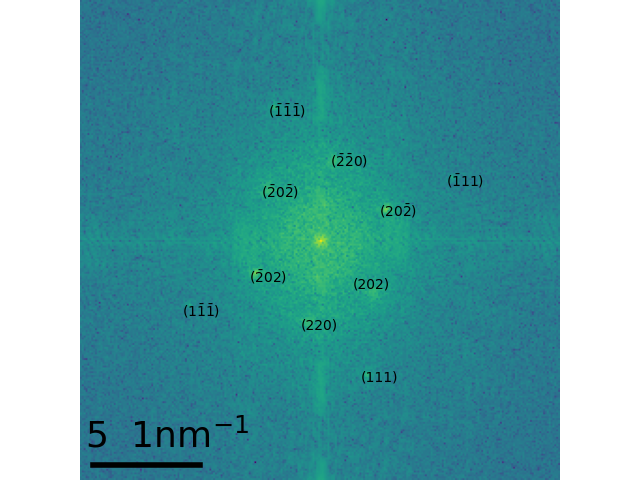
\includegraphics[scale=0.4]{../Graphics/caras.png}
    \caption{Transformada de Fourier de la figura \ref{fig:nanoparticula} con sus respectivos indices de Miller en cada punto de difracción.}
\end{figure}
En la figura \ref{fig:nanoparticula} y \ref{fig:lattice} se puede encontrar una estructura hexagononal, por lo cual se procedio a delimitar la zona hexagonoal, por lo que el resultado que se obtuvo es el siguient3:
\begin{figure}[H]
    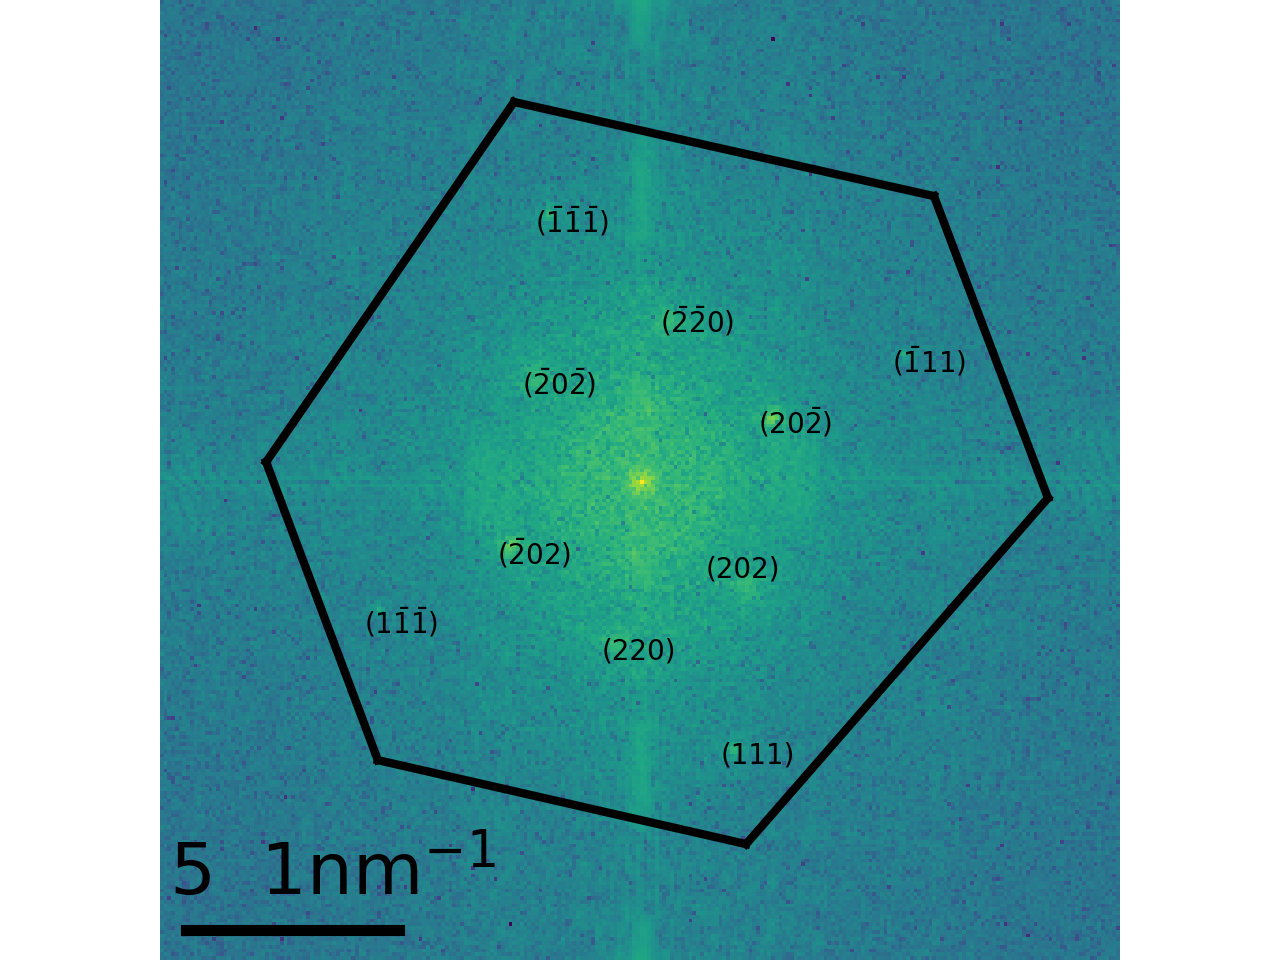
\includegraphics[scale=0.4]{../Graphics/hexa.png}
    \caption{Transformada de Fourier de la partícula de oro delimitada por la forma hexagonal.}
    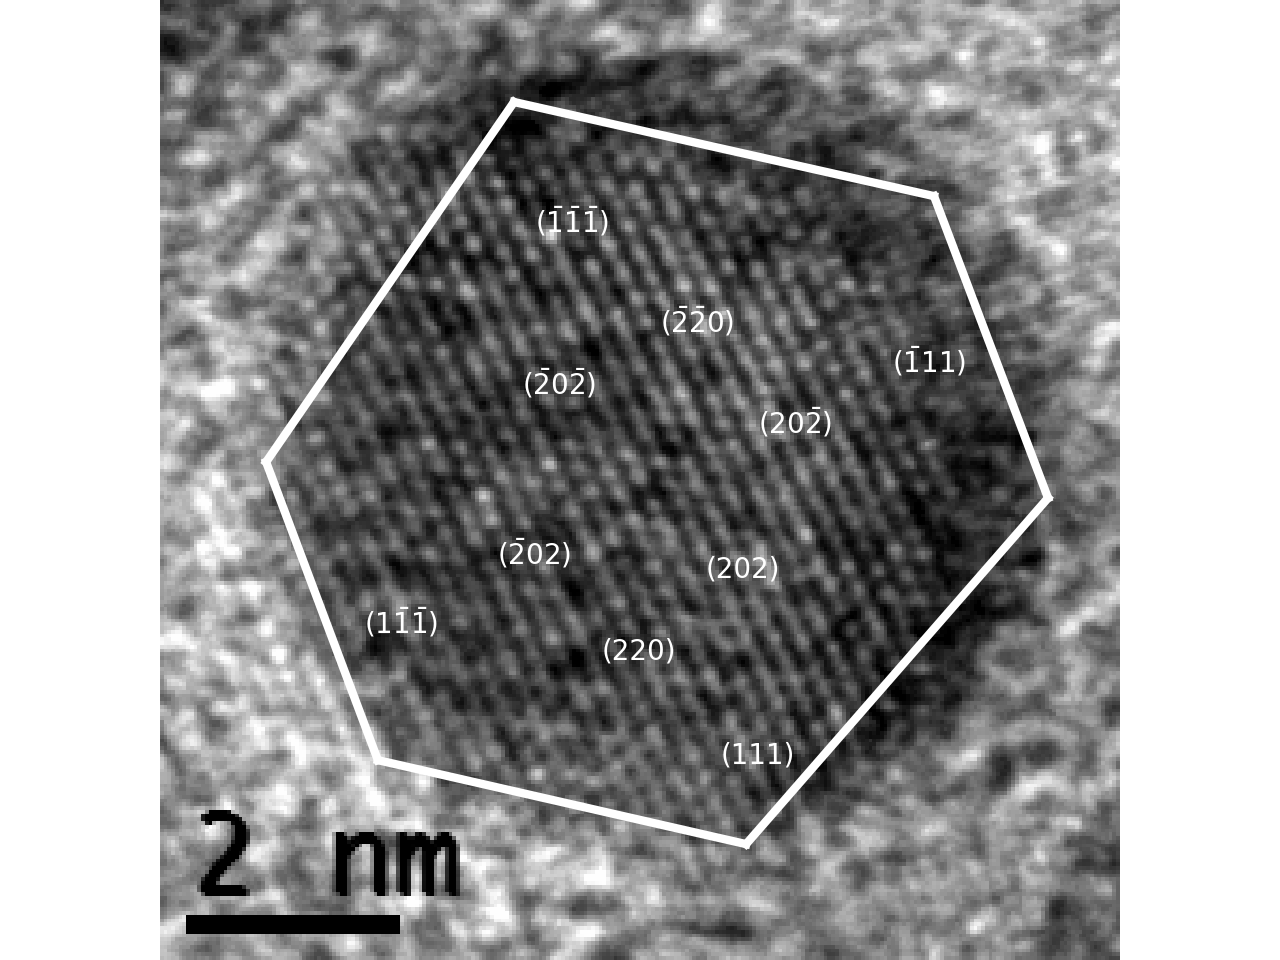
\includegraphics[scale=0.4]{../Graphics/nano_ind.png}
    \caption{Imagen de la nanopartícula de oro con sus indices de Miller indexados delimitados por la forma hexagonal encontrada.}
\end{figure}
\section{Conclusiones}
\section{Código}
\begin{itemize}
    \item \href{https://github.com/giovannilopez9808/Notas_Agosto_2020/blob/master/AMC/Reto2/FFT.py}{FFT.py}
    \item \href{https://github.com/giovannilopez9808/Notas_Agosto_2020/blob/master/AMC/Reto2/distancia.py}{distancia.py}
\end{itemize}
\bibliographystyle{plain}
\nocite{*}
\bibliography{Main}
\end{document}